\chapter{Numerical simulation of intact bioprosthetic heart valves}

\section*{Preface}
\addcontentsline{toc}{section}{Preface}%

  Bioprosthetic heart valves (BHVs), fabricated from exogenously crosslinked collagenous tissues, remain the most popular heart valve replacement design. However, the life span of BHVs remains limited to 10–15 years, in part because the mechanisms that underlie BHV failure remain poorly understood. The current process for evaluating BHV designs is an expensive and time consuming three-stage process: 1) accelerated wear testing(AWT), 2) large animal studies, and 3) clinical trials. AWT is currently the only way to evaluate BHV durability in a feasible amount of time (months instead of years). However, the loading conditions and environment during AWT are not physiological and the only durability information currently used is the presence of visible damage. Only the clinical evaluation stage can provide true indications of the \textit{in vivo} performance of BHV designs. However, this is the final, most difficult, most expensive and most time consuming stage. Clearly, current methods of evaluating BHV designs are not feasible for advancing the BHV technology in a timely manner. In this chapter, we implement our constitutive model for the time evolving properties of BHVs in response to permanent set developed in a previous chapter in a numerical simulation framework, and attempt to predict the geometric and structural change that occurs with the onset of permanent set. 




%---    INTRODUCTION
\section{Introduction}

\subsection{Background}
    The most popular replacement heart valves continue to be bioprosthetic heart valves (BHV) fabricated from xenograft biomaterials, for both established surgical and more novel percutaneous valve designs \cite{schoen_evolving_2008,schoen_new_2006,schoen_cardiac_2005,schoen_calcification_2005,schoen_pathology_2001}. While these devices have provided great benefits for many patients, device failure continues to be the result of leaflet structural deterioration mediated by fatigue and/or tissue mineralization \cite{vesely_tissue_2001,sacks_collagen_2002}. As a result, the life span of BHVs remains limited to 10–15 years, and the mechanisms that underlie such failures remain poorly understood. Thus, improved durability remains an important clinical goal and represents a unique cardiovascular engineering challenge resulting from the extreme valvular mechanical demands. Yet, current BHV assessments rely exclusively on device-level evaluations, which are confounded by simultaneous and highly coupled biomaterial mechanical fatigue, valve design, hemodynamics, and calcification. Thus, despite decades of clinical BHV usage and growing popularity, there exists no acceptable method for simulating BHV durability in any design context. While efforts to mitigate tissue mineralization have progressed well, efforts to minimize structural degradation remain limited. For example, in vitro accelerated wear tests (AWT) are used only for the most basic device level durability evaluations. Yet no systematic attempt has been made to glean important durability information from these required tests to inform mechanisms and means to simulate BHV durability. There is thus a profound need for the development of a novel simulation technologies for the prediction of the changes in the properties of BHVs to long-term cyclic loading.
    
    
\subsection{Mechanisms of BHV failure}

	The causes of BHV failure can be divided into two broad categories, mineralization and structural damage, with both processes occurring in parallel or independently \cite{sacks_collagen_2002}. Mineralization is the accumulation of mineral deposits, mainly calcium phosphate, within the BHV leaflets \cite{schoen_calcification_2005}. This disrupts the underlying microstructure preventing the proper mechanical function of BHVs, increasing the likelihood of tearing, and reducing flexibility (preventing normal opening and closing motions, and induce valve stenosis). The causes of calcification and associated anti-calcification treatments are extensively studied in literature \cite{park_novel_1997, isenburg_tannic_2005, vyavahare_prevention_1997}. On the other hand, structural damage includes the collagen fiber damage and breakdown of the non-fibrous part of extracellular matrix (ECM), \emph{which we will refer as simply the matrix}. Fourier transform infrared spectroscopy(FTIR) results have shown changes in the collagen fiber molecular structure after 50 million cycles \cite{sun_response_2004}, which suggests that some collagen fiber damage has occurred during this period. However, its effect on the mechanical response of BHVs was not detectable. Nevertheless, it is important to maintain the structural integrity of the BHV, as this will help to improve BHV durability.
	

\subsection{Constitutive model of BHV biomaterial under permanent set}

    In previous chapters, we developed a constitutive model for the underlying mechanical properties of collagenous soft tissues used to fabricate BHVs (Chapter 2, 3) as well as the extensions for the evolution of the material properties in response to permanent set (Chapter 4). The constitutive model utilizes the mechanisms at the meso-scale (i.e. at the level of the fiber, 10-100 $\mu$m in length scale), takes into account the layered structure of these tissue and the contributions from the distinct collagen and elastin fiber networks within each tissue layer to predict the mechanical response at the tissue scale. This approach was further extend for the effect of crosslinking on the fiber matrix interactions to simulate exogenously crosslinked materials. Requisite collagen and elastin fibrous structural information can be obtained using microscopy and conventional histology, and the approach was validated using a novel fibril-level (0.1 to 1 $\mu$m) approach to compare the predicted collagen fiber/fibril mechanical behavior with extant MV small angle X-ray scattering data. 
    
    
    Permanent set is the significant changes in geometry of BHVs observed in experimental studies \cite{smith_fatigue_1999}\cite{smith_high_1997} with in vivo operation. This can lead to stress concentrations that can have significant impact on structural damage. Structural damage was not detected in the time frame when permanent set is the most dominant. We hypothesize that the scission-healing reaction of glutaraldehyde is the underlying mechanism responsible for permanent set in exogenously crosslinked soft tissues. The continuous scission-healing process of glutaraldehyde allows a portion of the exogenously crosslinked matrix, which is considered to be the non-fibrous part of the extra-cellular matrix, to be re-crosslinked in the loaded state. We model the permanent set effect in chapter 4 by assuming that the exogenously crosslinked matrix undergoes changes in reference configurations over time. The changes in the collagen fiber architecture due to dimensional changes allow us to predict subsequent changes in mechanical response. A key finding we have is that the collagen fiber architecture has a limiting effect on the maximum changes in geometry that the permanent set effect can induce. This is due to the recruitment of collagen fibers as the changes in geometry due to permanent set increase. This means we can potentially optimize the BHV geometry based on the predicted the final BHV geometry after permanent set has largely ceased. 
    

\subsection{Numerical simulation framework}

    However, numerical simulations using our constitutive model for permanent set is quite costly. Due to the incorporation of the quadruple integral to calculate fiber interactions, the resulting computational cost is five magnitudes higher than conventional phenomenological approaches. It is for this reason that we developed an effective constitutive model for planar soft tissues, and a parameter estimation approach for rapidly determining the model parameters from the micro-model. This approach takes advantage of the computationally efficient forms of phenomenological models and the mechanisms and predictive capabilities of micro-models (meso-scale, multi-scale, or other complex constitutive models) (Fig. \ref{fig:simulationframework}A). For each iteration of the simulation, whether forward, inverse, or time-evolving, the effective constitutive model is first fit to the micro-model(s) to determine the model parameters, then it is used to performed the actual numerical simulation. Subsequent updates to the evolving material properties, geometry and boundary conditions are then performed (Fig. \ref{fig:simulationframework}B). This approach can greatly improve the computational efficiency of numerical simulations and make it possible for a finite element implementation of the permanent set simulation (Chapter 4). In this chapter, we develop and numerical simulation framework for the time evolving properties of BHVs in response to permanent set, and attempt to predict the geometric and structural change that occurs with long term cyclic loading. 
    
%%%%%%%%%%%%%%%%%%%%%%%%%%%%%%%%%%%%%%%%%%%%%%%%%%%%%%%%%%%%
%-------------------	begin FIGURE 	-------------------%
\begin{figure}
\centering
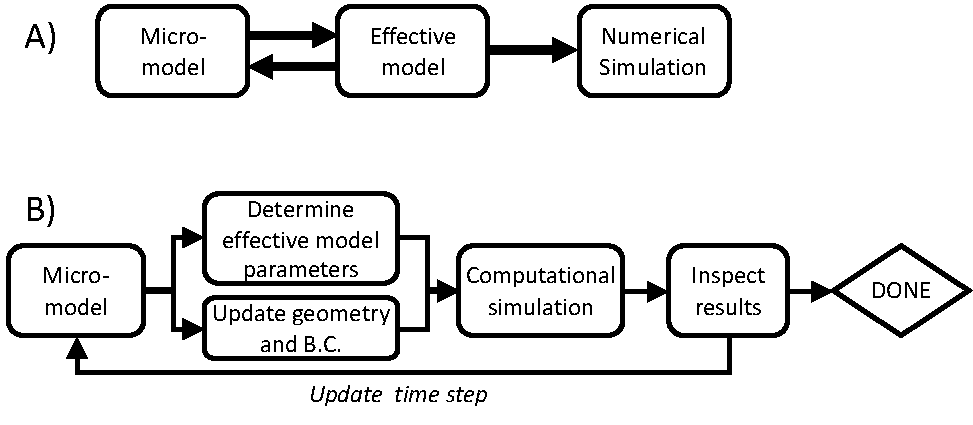
\includegraphics[width=\textwidth]{Images/chapter5/simulationframework}
\caption{Proposed frame work for using an effective constitutive model to improve the efficiency of using complex meso- or multi-scale models (micro\Hyphdash models) in numerical simulations. Here, A) effective constitutive models act as an intermediate step between micro-models and numerical simulations, where micro-models inform the changes to the effective constitutive model while the effective constitutive model for the simulation. B) An example of how this may be implemented for time\Hyphdash evolving is shown.}
\label{c6:fig:simulationframework}
\end{figure}
%-------------------	 end FIGURE 	-------------------%
%%%%%%%%%%%%%%%%%%%%%%%%%%%%%%%%%%%%%%%%%%%%%%%%%%%%%%%%%%%%
    
    

%---    METHODS
\section{Methods}

\subsection{Overall framework}

    To implement the permanent set model (chapter 4) for numerical simulations, we will utilize the effective constitutive model approach (chapter 5). This implementation has 4 main components (Fig. \ref{c6:fig:pssimoverview}): 1) initial state model, 2) quasistatic simulation, 3) updates to the material properties in response to permanent set and 4) updates to the finite element model geometry in response to permanent set. 
    
    
%%%%%%%%%%%%%%%%%%%%%%%%%%%%%%%%%%%%%%%%%%%%%%%%%%%%%%%%%%%%
%-------------------    begin FIGURE     -------------------%
\begin{figure}
\centering
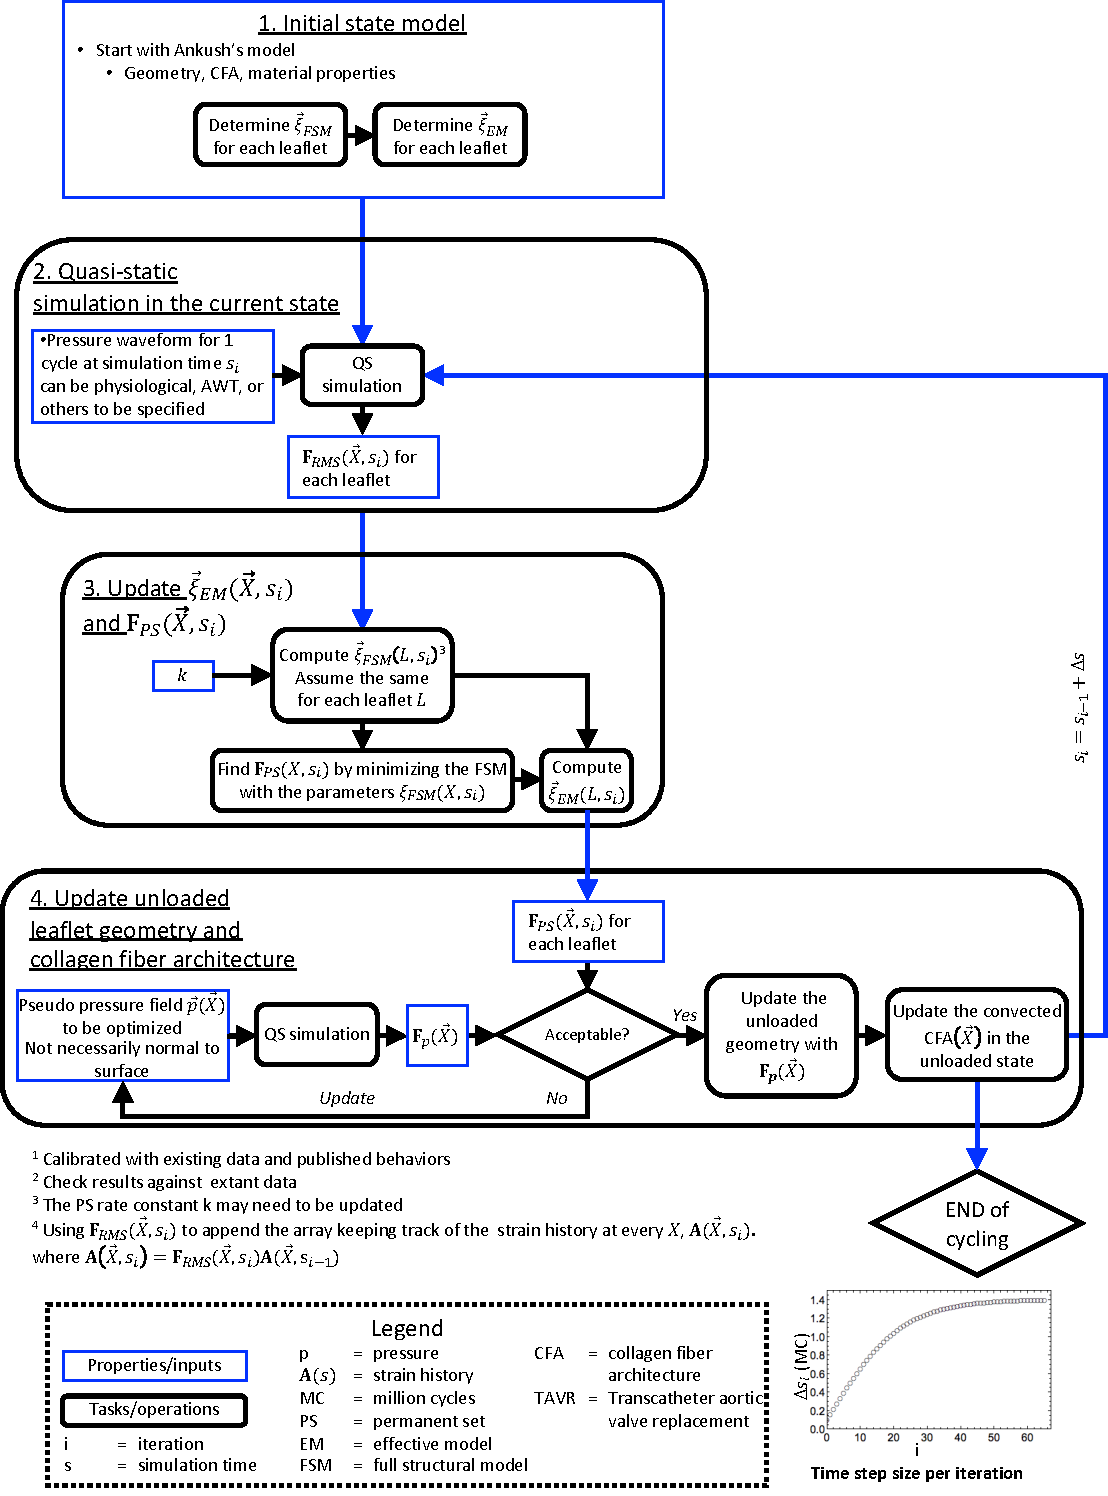
\includegraphics[width=5.5in]{Images/chapter6/pssimoverview.pdf}
\caption{Proposed framework for simulation the evolving properties of BHVs in response to permanent set.}
\label{c6:fig:pssimoverview}
\end{figure}
%-------------------     end FIGURE     -------------------%
%%%%%%%%%%%%%%%%%%%%%%%%%%%%%%%%%%%%%%%%%%%%%%%%%%%%%%%%%%%%

\subsection{Initial state model}

    In this part, the initial parameters of the simulation are established. The 3 main components are: 1) finite element mesh for BHV geometry, 2) leaflet material properties, and 3) mapped collagen fiber architecture. For the BHV geometry, our group developed a pipeline using micro-CT to measure the 3-dimensional geometry of the BHV and fitting the atrial surface points to a NURBS mesh using the grasshopper plugin in Rhino (Copyright Robert McNeel \& Associates) (Fig. \ref{c6:fig:fegeometry}). We also previously developed an approach for mapping the collagen fiber architecture to the finite element mesh \cite{aggarwal_patient_2013,aggarwal_inverse_2015}. However, due to the lack of available experimental data, we used the Edwards valve geometry from \cite{aggarwal_inverse_2015}, bovine pericardium material properties from \cite{sacks_novel_2015}, and circumferential aligned collagen fiber orientation distributions.
    
%%%%%%%%%%%%%%%%%%%%%%%%%%%%%%%%%%%%%%%%%%%%%%%%%%%%%%%%%%%%
%-------------------    begin FIGURE     -------------------%
\begin{figure}
\centering
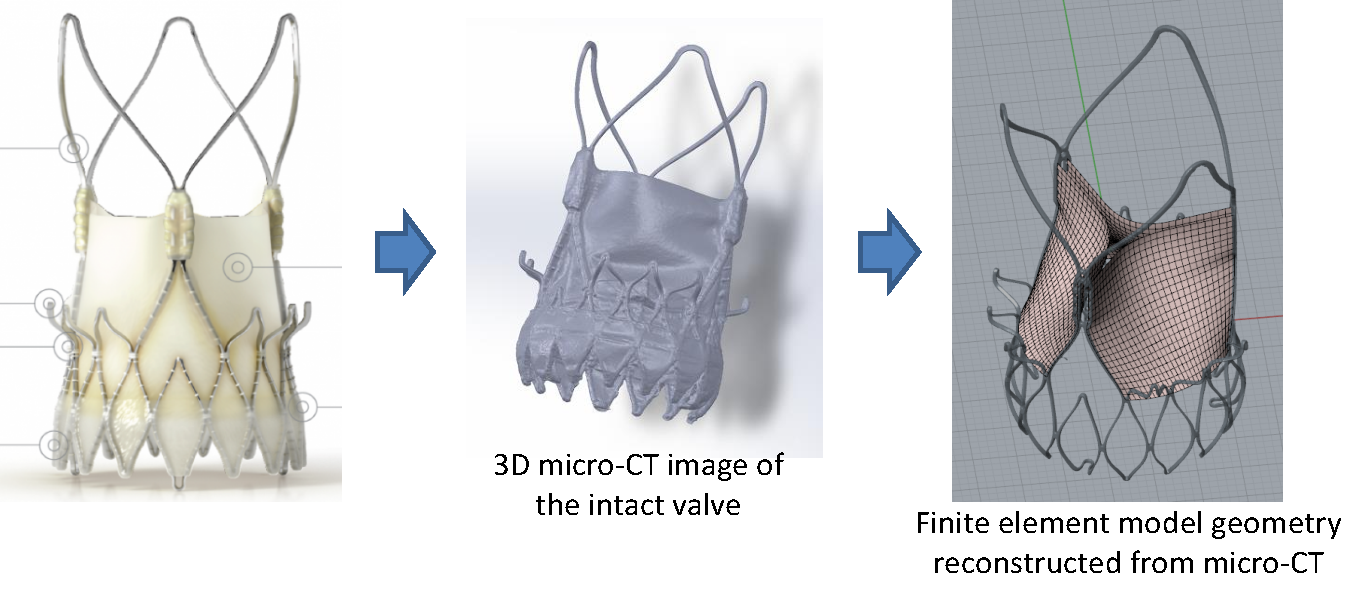
\includegraphics[width=5.5in]{Images/chapter6/fegeometry.pdf}
\caption{Pipeline for converting micro-CT data for each reference and loading states to finite element meshes and geometry.}
\label{c6:fig:fegeometry}
\end{figure}
%-------------------     end FIGURE     -------------------%
%%%%%%%%%%%%%%%%%%%%%%%%%%%%%%%%%%%%%%%%%%%%%%%%%%%%%%%%%%%%

\subsection{Quasistatic simulation of bioprosthetic heart valves}

    For the quasistatic simulation, which is necessary to determine the current loaded state, we will utilize the effective model approach (Fig. \ref{c6:fig:simulationframework}) established in chapter 5. For finite element model, we utilized the custom finite element simulation software developed by Hsu \textit{et al.} \cite{hsu_dynamic_2015, kamensky_immersogeometric_2015, kiendl_isogeometric_2015, wu_anisotropic_2018}. Briefly, the finite element code was developed for isogeometric fluid-solid dynamics simulation of heart valves, focusing mostly on the tri-leaflet atrioventricular valves. The tri-leaflet geometry is based on the commonly used Edwards Pericardial Heart Valve with Kirchhoff-Love shells for the leaflets \cite{kiendl_isogeometric_2015} and finite element solver developed in by Kamensky \textit{et al.} \cite {kamensky_immersogeometric_2015}. We utilized this code to simulate leaflet deformation under physiological quasi-static transvalvular pressure. 
    A total was 484 B\'ezier elements was used for each leaflet, with a leaflet density of 1.0 g/cm$^3$ and a uniform leaflet thickness of 0.386mm thick \cite{hsu_dynamic_2015}. Contact between leaflets is handled by a penalty-based approach and imposed at quadrature points of the shell structure, and clamped boundary condition is applied to the leaflet attachment edge. 
    For simplicity and consistency, the collagen fiber direction was assumed to be aligned to the circumferential direction of each leaflet. No root, atrial chamber or the surrounding artery was used. The bioprosthetic heart valve stent was made rigid and undeformable, serving a stationary reference for the leaflets. A similar validation process to the one presented by Wu \textit{et al.} \cite{wu_anisotropic_2018} to verify the implementation.
    
    
    For the constitutive model for the leaflet material, we used the effective material model (chapter 5)
	%==========================================================%
%-------------------	begin EQUATION 	-------------------%
\begin{equation} \label{c6:eqn:finalexponentialmodelformscaled}
\begin{aligned}
\Psi_{eff} 	=& c_0 \left(e^{Q} - 1\right) = c_0^\prime e^{-Q_{max}}\left(e^{Q} - 1\right)    \\
Q		=& b_1 E_m^2 + b_2 E_n^2 + b_3 E_\phi^2 + b_4 E_m E_n + b_5 E_m^4 + b_6 E_n^4 + b_7 E_m^3 E_n + b_8 E_m^2 E_n^2 \\ 
&+ b_9 E_m E_n^3 + b_{10} E_\phi^4 + b_{11} E_m^2E_\phi^2 + b_{12} E_n^2 E_\phi^2 + b_{13} E_m E_n E_\phi^2 \\
Q		=& b_1 (E_m^{max})^2 + b_2 (E_n^{max})^2 + b_3 (E_\phi^{max})^2 + b_4 (E_m^{max}) (E_n^{max}) + b_5 (E_m^{max})^4   \\
    &+ b_6 (E_n^{max})^4 + b_7 (E_m^{max})^3 (E_n^{max}) + b_8 (E_m^{max})^2 (E_n^{max})^2 + b_9 (E_m^{max}) (E_n^{max})^3	\\
	&+ b_{10} (E_\phi^{max})^4 + b_{11} (E_m^{max})^2(E_\phi^{max})^2 + b_{12} (E_n^{max})^2 (E_\phi^{max})^2    \\ 
	&+ b_{13} (E_m^{max}) (E_n^{max}) (E_\phi^{max})^2,
\end{aligned}
\end{equation}
%-------------------	 end EQUATION 	-------------------%
%==========================================================%
	to homogenize the mechanical response of the permanent set model. The resulting elasticity tensor can be found in Appendix \ref{sec:elasticitytensor}, Eqn. \ref{eqn:greenelasticityform}). To test the finite element implementation, and the effective constitutive model approaches, we performed several quasi-static simulations of BHVs with different leaflet materials properties. The main properties considered are bovine pericardium (most commonly used for bioprosthetic heart valve leaflets), porcine aortic valve (highly anisotropy response), and bovine pericardium with a uniform fiber ODF (isotropic). We replicated the response of these tissues using the static part of the permanent set constitutive model for collagenous soft tissues (Eqn. \ref{c6:eq:fullEXLmodel}) based on their microstructure. We then fit $\Psi_{eff}$ (Eqn. \ref{c6:eqn:finalexponentialmodelformscaled}) their response by sampling along optimal loading paths. Next, we evaluated the computational cost and numerical robustness of $\Psi_{eff}$ and its ability to handle a wide range of material properties and the complex \textit{in vivo} deformations in numerical simulations.
    

\subsection{Constitutive model for the evolving material properties under permanent set}

    The detailed theory for the constitutive model for permanent set is presented in chapter 4. Briefly, the constitutive model consists of three parts: collagen, matrix, and interactions,
%==========================================================%
%-------------------    begin EQUATION     -------------------%
\begin{equation}
\Psi     = \Psi_\mathrm{col} + \Psi_\mathrm{mat} + \Psi_\mathrm{int} \label{c6:eqn:structuralmodelcomponents}. 
\end{equation}
%-------------------     end EQUATION     -------------------%
%==========================================================%
    The time evolving mechanism is based on the work by Rajagopal and Wineman \cite{rajagopal_constitutive_1992}, where we assume that the response of the EXL matrix is a constrained mixture model consisting of the origin fraction being continuously converted to new fractions with a reference state in the current loaded configuration. 
\begin{equation} \label{c6:eq:wineman}
\phi_m \mathbf{S}_m = b(s)\mathbf{\bar{S}}_m^\mathrm{existing} + \int\displaylimits_0^s a(s,\hat{s})\mathbf{\bar{S}}_m^\mathrm{new} \mathrm{d}\hat{s},
\end{equation}

    The final model form as a function of the permanent set rate constant $k $, the permanent set deformation $\mathbf{F}_\mathrm{PS}$, the strain history $\mathbf{A}(s)$, and the material parameters of the constitutive model in the uncycled state. The input of the model is the applied deformation $\mathbf{C}$ referenced to the current unloaded state $\Omega_\mathrm{PS}$, given by the deformation $\mathbf{F}_\mathrm{PS}$ from $\Omega_0$. The full form is
\begin{equation}\label{c6:eq:fullEXLmodel}
\mathbf{S} = \mathbf{S}\left(k , \mathbf{F}_\mathrm{PS}, \mathbf{A}(\hat{s}), \mathbf{C}\right) = \phi_\mathrm{col} \left[ \mathbf{S}_\mathrm{col} + \mathbf{S}_\mathrm{int}\right] + \phi_m \mathbf{S}_\mathrm{m},
\end{equation}
where the collagen contribution is 
\begin{equation} \label{c6:eq:fullcollagen}
\begin{split}
\phi_\mathrm{col}\mathbf{S}_\mathrm{col}&\left(k , \mathbf{F}_\mathrm{PS}, \mathbf{A}(\hat{s}), \mathbf{C}\right) \\
&= \phi_\mathrm{col} \eta_C \int\displaylimits_\theta \Gamma_1(\mathbf{F}_{\mathrm{PS}}, \theta)\left\lbrace 
\int\displaylimits_1^{\lambda_\theta} \frac{D_1\left( \mathbf{F}_{\mathrm{PS}}, x \right)}{x} \left( \frac{1}{x}- \frac{1}{\lambda_\theta}\right) \mathrm{d}x \right\rbrace \mathbf{n}_\theta\otimes\mathbf{n}_\theta \mathrm{d}\theta,
\end{split}
\end{equation}
where $\lambda_\theta = \sqrt{\mathbf{n}_\theta \cdot \mathbf{C}\mathbf{n}_\theta}$ is the stretch of the fiber ensemble oriented along $\theta$, the fiber ensemble interactions is 
\begin{equation} \label{c6:eq:fullinteractions}
\begin{split}
\phi_\mathrm{int}\mathbf{S}_\mathrm{int}&\left(k , \mathbf{F}_\mathrm{PS}, \mathbf{A}(\hat{s}), \mathbf{C}\right) \\
=& \phi_\mathrm{col} \eta_\mathrm{int} \int\displaylimits_\alpha \int\displaylimits_\beta \Gamma_1 \left(\mathbf{F}_\mathrm{PS}, \alpha \right) \Gamma_1 \left(\mathbf{F}_\mathrm{PS},  \beta \right) \\
&\times\left[ \left\lbrace 
\int\displaylimits_1^{\lambda_\alpha} \int\displaylimits_1^{\lambda_\beta} 
\frac{2 \lambda_\beta D_1(\mathbf{F}_\mathrm{PS}, x_\alpha) D_1(\mathbf{F}_\mathrm{PS}, x_\beta)}{x_\alpha x_\beta} 
\left( \frac{\lambda_\alpha}{x_\alpha} \frac{\lambda_\beta}{x_\beta} - 1\right) \mathrm{d}x_\alpha \, \mathrm{d}x_\beta \right.\right. \\
&+ \left. \left. \int\displaylimits_1^{\lambda_\beta} D_1(\mathbf{F}_\mathrm{PS}, x_\beta) \left( \frac{\lambda_\beta}{x_\beta} -1  \right)^2 \mathrm{d}x_\beta \right\rbrace \right.  \frac{\mathbf{n}_\alpha \otimes \mathbf{n}_\alpha}{\lambda_\alpha}  \\
&+ \left. \left\lbrace
\int\displaylimits_1^{\lambda_\alpha} \int\displaylimits_1^{\lambda_\alpha} 
\frac{2 \lambda_\beta D_1(\mathbf{F}_\mathrm{PS}, x_\alpha) D_1(\mathbf{F}_\mathrm{PS}, x_\beta)}{x_\alpha x_\beta} 
\left( \frac{\lambda_\alpha}{x_\alpha} \frac{\lambda_\beta}{x_\beta} - 1\right) \mathrm{d}x_\alpha \, \mathrm{d}x_\beta 
\right. \right. \\
&+\left. \left. \int\displaylimits_1^{\lambda_\alpha} D_1(\mathbf{F}_\mathrm{PS}, x_\alpha) \left( \frac{\lambda_\alpha}{x_\alpha} -1  \right)^2 \mathrm{d}x_\alpha \right\rbrace \frac{\mathbf{n}_\beta \otimes \mathbf{n}_\beta}{\lambda_\beta}  \right] \mathrm{d}\alpha \, \mathrm{d}\beta,
\end{split}
\end{equation}
and the EXL matrix is
\begin{equation} \label{c6:eq:fullmatrix}
\begin{split}
\phi_m \mathbf{S}_\mathrm{m}&\left(k , \mathbf{F}_\mathrm{PS}, \mathbf{A}(\hat{s}), \mathbf{C}\right) \\
&= \phi_m \eta_m \left[ \vphantom{\int\displaylimits_0^s} \mathrm{Exp}\left[-k  \cdot s\right]  \left(\left( \bar{I_1} (\mathbf{F}_\mathrm{PS}, \mathbf{A}(0)) - 3\right)^{\alpha - 1} + r \left( \bar{I_1} (\mathbf{F}_\mathrm{PS}, \mathbf{A}(0)) - 3\right)^{\beta - 1}\right)  \right.\\
&\times \left( \mathbf{\tilde{B}}(\mathbf{F}_\mathrm{PS}, \mathbf{A}(0))^{-1} - \tilde{B}_{33}^{-1}(\mathbf{F}_\mathrm{PS}, \mathbf{A}(0))C_{33}\mathbf{C}^{-1}\right) \\
&+ \int\displaylimits_0^s k \cdot \mathrm{Exp}\left[-k (s - \hat{s})\right] \left(\left( \bar{I_1} (\mathbf{F}_\mathrm{PS}, \mathbf{A}(\hat{s})) - 3\right)^{\alpha - 1} + r \left( \bar{I_1} (\mathbf{F}_\mathrm{PS}, \mathbf{A}(\hat{s})) - 3\right)^{\beta - 1}\right) \\
&\times \left. \vphantom{\int\displaylimits_-^s} \left( \mathbf{\tilde{B}}(\mathbf{F}_\mathrm{PS}, \mathbf{A}(\hat{s}))^{-1} - \tilde{B}_{33}^{-1}(\mathbf{F}_\mathrm{PS}, \mathbf{A}(\hat{s}))C_{33}\mathbf{C}^{-1}\right) \mathrm{d}\hat{s}\right].
\end{split}
\end{equation}

\subsection{Geometry update in response to permanent set}

    Although the permanent set model can find the local change in reference geometry, ($\mathbf{F}_\mathrm{PS}$), can be determined from equation \ref{c6:eq:fullmatrix} using
\begin{equation}\label{c6:eq:optimization}
\begin{gathered}
\mathbf{F}_\mathrm{PS} = \operatorname*{arg\,min}_\mathbf{F} \left\Vert \mathbf{S}\left(k , \mathbf{I}, \mathbf{A}(\hat{s}), \mathbf{C}=\mathbf{F}^\mathsf{T}\mathbf{F}\right) - 0 \right\Vert.
\end{gathered}
\end{equation}
    This is only local and will not be sufficient for generating a compatible mesh. To generate the updated reference configuration, we will do this by simulation. First the local change in geometry is found (Eqn. \ref{c6:eq:optimization}). Next, we will compute an equivalent stress using equation \ref{c6:eq:fullEXLmodel}, by
\begin{equation}\label{c6:eq:psstress}
\begin{gathered}
\mathbf{S}_\mathrm{PS} = \mathbf{S}(\mathbf{F}_\mathrm{PS}).
\end{gathered}
\end{equation}
    This permanent set stress, $\mathbf{S}_\mathrm{PS}$, is equivalent of a growth stress, which is then added to the weak form presented in equation 1 of Wu et al. \cite{wu_anisotropic_2018} as 
\begin{equation}\label{c6:eq:weakform}
\begin{aligned}
\int_{\Gamma_0} \mathbf{w}\cdot\rho h_{th} \left.\dpd[2]{y}{t}\right|_\mathbf{X} \dif\Gamma + 
\int_{\Gamma_0} \int_{-h_{th}/2}^{h_{th}/2}\delta\mathbf{E}:(\mathbf{S} + \mathbf{S}_\mathrm{PS}) \dif \xi^3\dif\Gamma&  \\
- \int_{\gamma_0} \mathbf{w}\cdot\rho h_{th}\mathbf{f}\dif\Gamma -\int_{\Gamma_t} \mathbf{w}\cdot\mathbf{h}\dif\Gamma = 0&
\end{aligned}
\end{equation}   
    The resulting control point displacements are then added to the finite element mesh from the previous time step to generate the new mesh in the new reference configuration. 
    

\subsection{Complete implementations with Python wrapper}

    The complete implementation of the time evolving simulation is done using a Python3 wrapper (Fig. \ref{c6:fig:pythonimplementation}) of the different components: 
    \begin{enumerate}[label=\Alph*]
        \item Quasi-static (QS) simulation code to obtain the NURBS control point displacement data for different loading conditions
        \item A post processor for translate displacement data to strain data at each gauss point
        \item The constitutive model for determining the change in material properties due to permanent set gauss point
        \item Parameter estimation code for determining the effective model parameters at each time step and gauss point
        \item Python code for updating the NURBS finite element mesh after each time step
        \item Python code for updating the collagen fiber orientation after each time step
    \end{enumerate}
    To start, we will use the Edwards valve geometry from \cite{aggarwal_inverse_2015}, bovine pericardium material properties from \cite{sacks_novel_2015}, and circumferential aligned collagen fiber orientation distributions. Next, the following process is iterated:
    \begin{enumerate}
        \item Perform QS simulation using the finite element code to determine the loading state
        \item Using the post processor to convert control point displacement data to local strain data, $\mathbf{A}(\Hat{s})$, at the current time $\Hat{s}$
        \item Append the strain in the loaded configuration, $\mathbf{A}(\Hat{s})$, to the full strain history $\mathbf{A}(s)$
        \item Update the permanent set constitutive model (Eqn. \ref{c6:eq:fullEXLmodel})
        \item Use equation \ref{c6:eq:fullEXLmodel} to compute the local $\mathbf{F}_\mathrm{PS}$, 
        $\mathbf{S}_\mathrm{PS}$, and mechanical data along optimal loading paths (chapter \ref{sec:optimaldesign})
        \item Use the local permanent set deformation to convect the collagen fiber orientation distribution $\Gamma_i$ in the current state to $\Gamma_{i+1}$ in the post permanent set state using 
        %-------------------    begin EQUATION     -------------------%
        \begin{equation}\label{c6:eqn:45}
        \begin{aligned}
        \Gamma_{i+1}[\mu_\Gamma,\sigma_\Gamma, \theta_{i+1}] = \Gamma_i[\mu_\Gamma, \sigma_\Gamma, \theta_i(\prescript{i+1}{i}{\mathbf{F}},\theta_{1+1})\frac{\prescript{i+1}{i}{\lambda}_{\theta_i}^2}{\prescript{i+1}{i}{J_\mathrm{2D}}}].
        \end{aligned}
        \end{equation}
        %-------------------     end EQUATION     -------------------%
        Note that the angle $\theta_1$ of a fibre originally oriented at $\theta_0$ can be determined using
        %-------------------    begin EQUATION     -------------------%
        \begin{equation}\label{c6:eqn:46}
        \begin{aligned}
        \theta_{i+1}(\prescript{i+1}{0i}{\mathbf{F}},\theta_i) = \tan^{-1}\left(\frac{\prescript{i+1}{i}{F}_{21}\cos{\theta_i} + \prescript{i+1}{i}{F}_{22}\sin{\theta_i}}{\prescript{i+1}{i}{F}_{11}\cos{\theta_i} + \prescript{i+1}{i}{F}_{12}\sin{\theta_i}}\right)
        \end{aligned}
        \end{equation}
        %-------------------     end EQUATION     -------------------%
        \item[7a] Perform QS simulation using the finite element code with $\mathbf{S}_\mathrm{PS}$ as the loading condition
        \item[7b] Added the control point displacement data to the current mesh geometry
        \item[8] Determine the new effective constitutive model parameters by performing parameter estimation on the optimal loading path data using equation \ref{c6:eqn:finalexponentialmodelformscaled}
        \item[9] Go to step 1 and rerun the QS simulation using the new mesh geometry, effective constitutive model parameters, and collagen fiber architecture
    \end{enumerate}
    This loop is run for the desired number of cycles. 
%%%%%%%%%%%%%%%%%%%%%%%%%%%%%%%%%%%%%%%%%%%%%%%%%%%%%%%%%%%%
%-------------------	begin FIGURE 	-------------------%
\begin{sidewaysfigure}
\centering
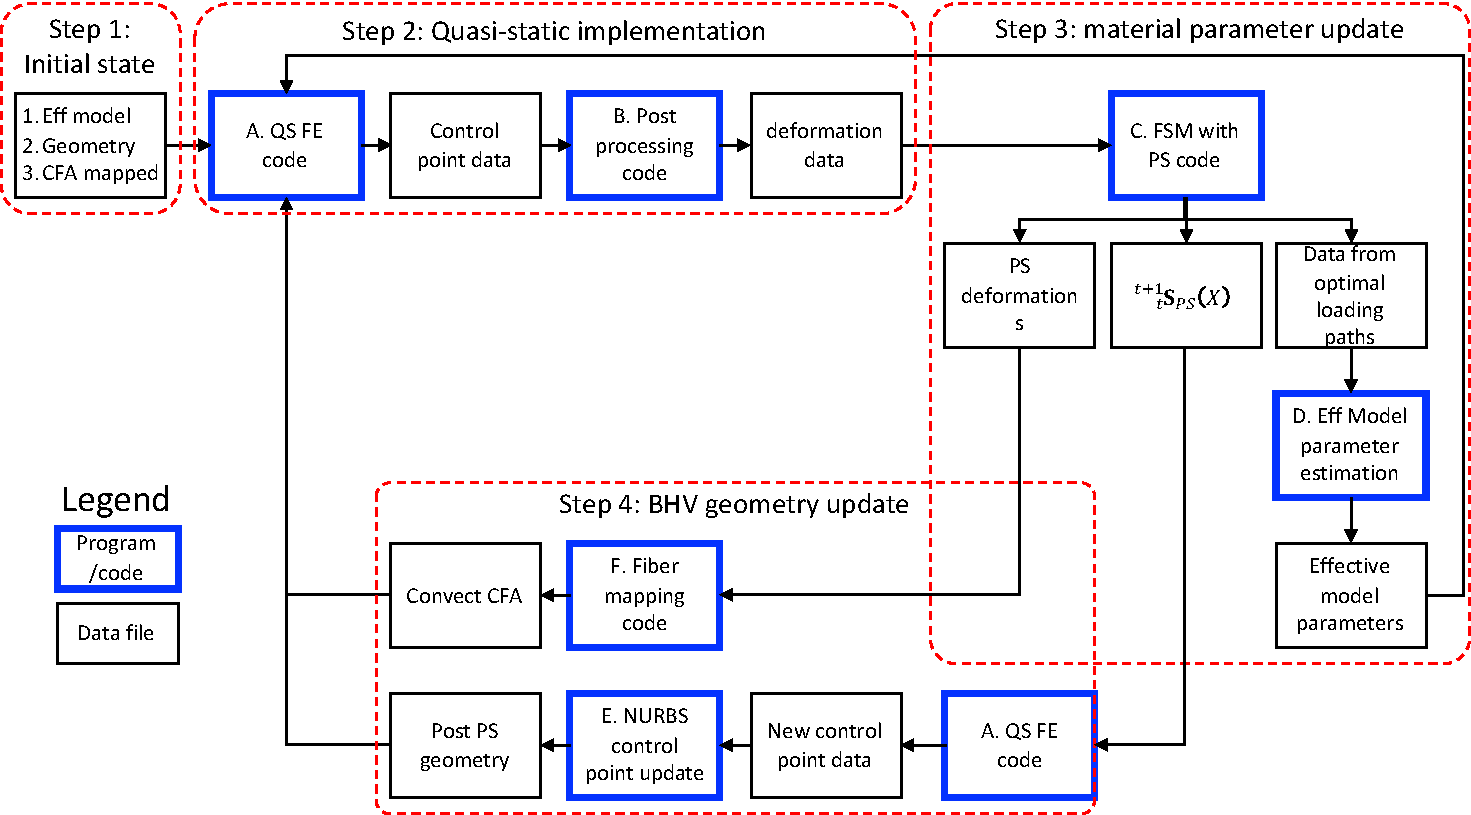
\includegraphics[width=8.2in]{Images/chapter6/pythonimplementation.pdf}
\caption{The python wrapper for communicating and execution of the different component of the time dependent simulation framework.}
\label{c6:fig:pythonimplementation}
\end{sidewaysfigure}
%-------------------	 end FIGURE 	-------------------%
%%%%%%%%%%%%%%%%%%%%%%%%%%%%%%%%%%%%%%%%%%%%%%%%%%%%%%%%%%%%

%---    Results
\section{Results and discussion}


%%%%%%%%%%%%%%%%%%%%%%%%%%%%%%%%%%%%%%%%%%%%%%%%%%%%%%%%%%%%%
%%  Application to numerical simulations of BHVs under      %
%   quasistatic loading                                     %

\subsection{Numerical simulation of bioprosthetic heart valve deformation}
	
    Planar biaxial test simulations were conducted to ensure that $\Psi_{eff}$ (Eqn. \ref{c6:eqn:finalexponentialmodelformscaled}) and the elasticity tensor (Appendix \ref{sec:elasticitytensor}, Eqn. \ref{eqn:greenelasticityform}) were properly implemented in the finite element simulation framework.  We compared the computation time for both $\Psi_{eff}$ and Holzapfel-Gasser-Ogden model for biaxial simulation of bioprosthetic heart valve tissues and expectedly found no significant increase in computational cost. The total elapsed time for $\Psi_{eff}$ is 7.58 seconds in comparison to 6.40 seconds for the Holzapfel-Gasser-Ogden model, much faster than any micro-models can achieve.  

	Next we simulated tri-leaflet valves with model parameters derived from bovine pericardium, porcine aortic valve leaflet, and an idealized isotropic case. This is a simple demonstration of the use of the $\Psi_{eff}$ for the upscaling and homogenizing of micro-models. The model parameters for the bovine pericardium case were derived from the simplified structural model and model parameter of Aggarwal and Sacks \cite{aggarwal_inverse_2015}, and the resulting response matched very well qualitatively. Due to a lack of fiber mapping in the quasi-static simulation software used, some minor difference are still expected. We found no difficulty when simulating the pericardium, aortic, or isotropic valves. Suggesting that $\Psi_{eff}$ is quite robust numerically.
	
	
\begin{figure}
\centering
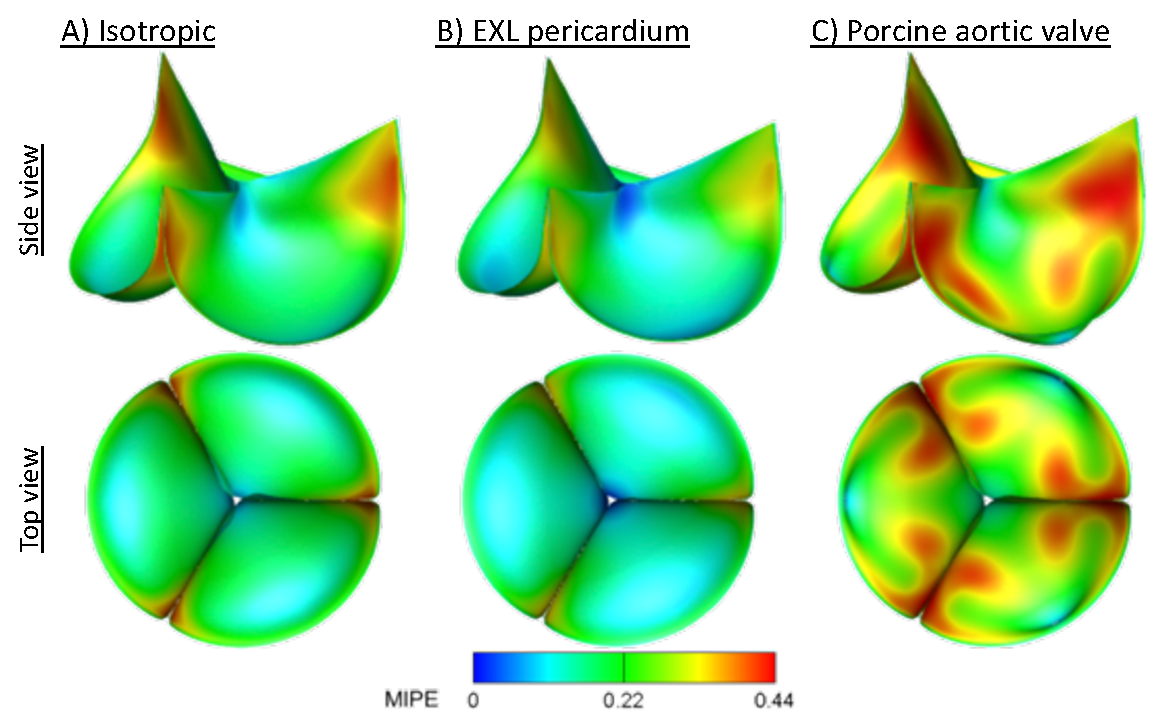
\includegraphics[width=\textwidth]{Images/chapter5/valvesimulations}
\caption{Simulations of intact tri-leaflet valves using A) the porcine aortic valve properties with an uniform fiber orientation distribution, B) exogenously cross-linked bovine pericardium properties with the most homogenous stress distribution, and C) the porcine aortic valve properties properties which results in a very heterogeneous stress distribution and the belly region caving in. The top row shows the side view of the valves at 80 mmHg and the bottom row shows the top-down view of the valves at the same transvalvular pressure.}
\label{fig:valvesimulations}
\end{figure}
    
    The material properties have significant effects on the mechanical behaviors of the leaflets (Fig. \ref{fig:valvesimulations}). The strain distributions within the leaflets were obtained for the pressure-loaded, fully-closed configurations of the valve, and then plotted with the maximum in plane Green-Lagrange strain (MIPE). When comparing the three different material, we can see that the native aortic valve properties result in significant heterogeneities in the deformation of the leaflets (Fig. \ref{fig:valvesimulations}C). Specifically, the belly region of the leaflets significantly protrudes out, increasing the load in the surrounding regions, especially near the commissures. This results in some stress concentrations that are not conducive to heart valve durability and health in general. The bovine pericardium valve (Fig. \ref{fig:valvesimulations}B) and the isotropic valve (Fig. \ref{fig:valvesimulations}A) on the other hand have significantly more homogeneous leaflet deformations, especially from the top-down view. Both of these undergo approximately the same deformation of 0.2 in MIPE. The largest difference between the two is near the commissure regions of the valve. Where the isotropic case is under significantly higher strain. Functionally, the material properties of the exogenously cross-linked bovine pericardium are the most suitable for heart valve leaflets, which distributes the stresses more evenly. 
    
    Much of the reasons behind these differences are likely to be due to the differences between the apparent mechanical properties \textit{in vivo} and the measured mechanical response in the laboratory setting. This is especially true for the aortic valve, which is extremely anisotropic with very high compliance in the radial direction of the leaflets. This difference is most likely due to the mismatch of referential configuration between the two states. Residual strain or residual stress has significant impact on the functional properties of the leaflets, specifically the apparent anisotropy and stiffness. Collagen fiber directions and varying regional properties can also have significant impact on the functional properties of the leaflets, and thus the results of the simulation. The valve leaflet shape, root geometry and properties, the arterial or ventricular geometry and loading conditions, can all be significant factors affecting the functions and stress distribution of the valve leaflets. Furthermore, how these factors affect the fluid dynamics of the valves is also an interesting question, suitable for further study. All in all, this is meant to be a demonstration and proof of concept for using $\Psi_{eff}$ to handle a wide range of soft tissue behaviors and anisotropy for the simulation of biological organs, in this case heart valves. Further and more detailed studies will be reserved for the future.  



\subsection{Permanent set simulation of bioprosthetic heart valve}
    This initial was done with 1) homogenous material parameters simular to bovine pericardium from Sacks and Zhang \cite{sacks_novel_2016}, 2) the Edward valve geometry from \cite{aggarwal_inverse_2015}, and collagen fiber distributions aligned with the circumference direction and a standard deviation of $30^\circ$. The key result is that permanent set slow done after around 20 million cycles and nearly completely seizes after 30 million cycles (Fig. \ref{c6:fig:psdeformation} \&\ref{c6:fig:psnoi}). This effect is closely linked the microstructural of the collagen fiber network. The gradual slow down is correlated with the straightening and recruitment of collagen fibers. This was predicted from the constitutive model (Eqn. \ref{c6:eq:fullEXLmodel}) (Fig. \ref{fig:parametric}). This is an important structural response, which allows us to predict the final reference geometry of the BHV. Since 30 million cycles corresponds to only 1 year after being surgically implanted, the BHV will remain in this configuration for the rest of its 9-14 year life span. By optimizing the initial BHV design so that the peak stress is minimal in the configuration after permanent set has seized, we can potentially improve the durability of BHVs by minimizing the load on the collagen fibers. Because collagen fibers have high rates of failure after being extended by 7-8\% \cite{lanir_structural_1979}\cite{buehler_atomistic_2006}, more evenly distributing the stresses can reduce this mode of failure. 
    
%%%%%%%%%%%%%%%%%%%%%%%%%%%%%%%%%%%%%%%%%%%%%%%%%%%%%%%%%%%%
%-------------------	begin FIGURE 	-------------------%
\begin{figure}
\centering
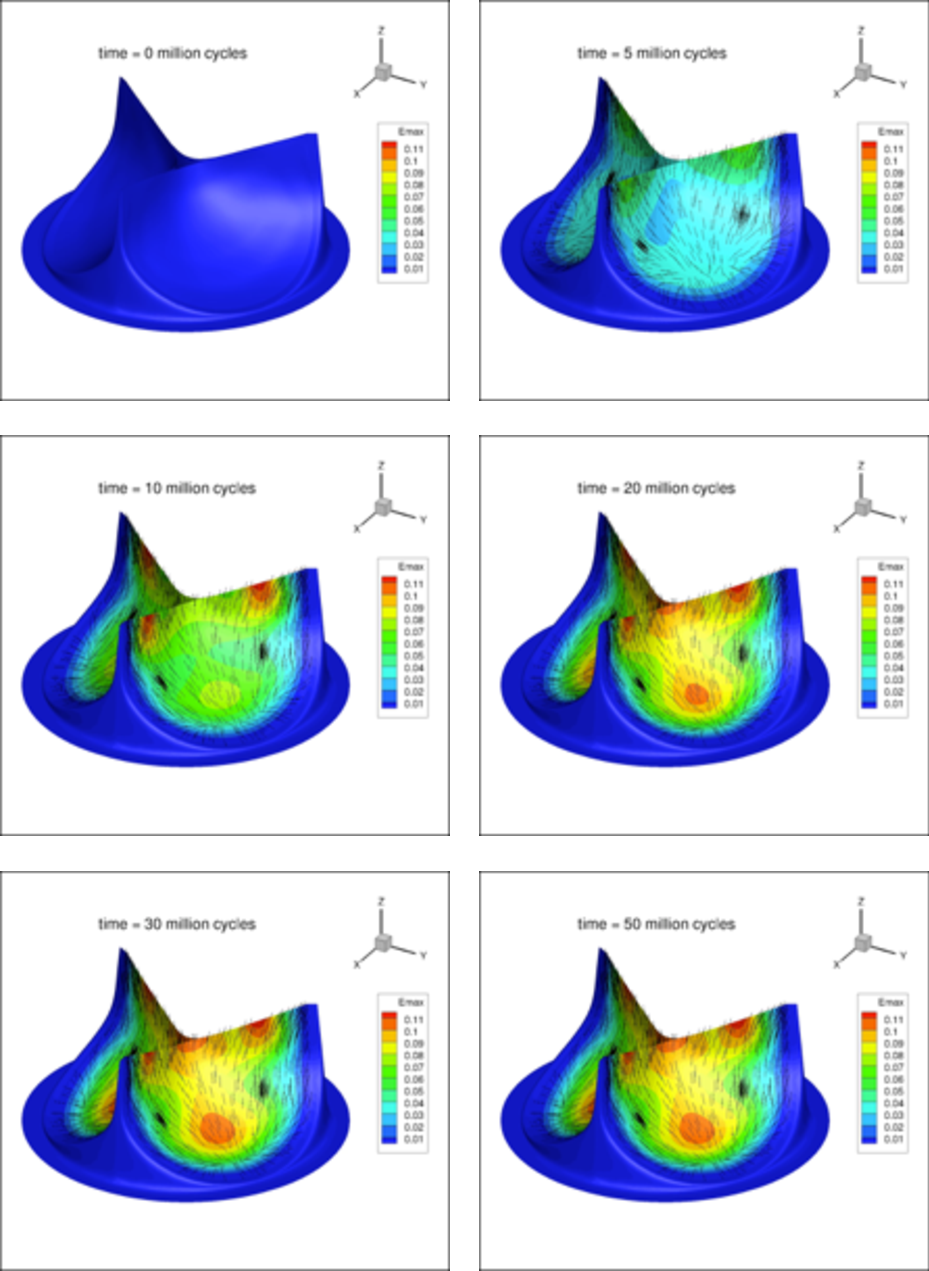
\includegraphics[width=5in]{Images/chapter6/psdeformation.pdf}
\caption{The simulation of the evolution of the referential configuration with the maximum principal in\Hyphdash plane Green-Lagrange strain (MIPE) overlayed on top at different cycle levels. Colors indicate the magnitude of MIPE, and the lines indicate the principal direction of the permanent set deformation.}
\label{c6:fig:psdeformation}
\end{figure}
%-------------------	 end FIGURE 	-------------------%
%%%%%%%%%%%%%%%%%%%%%%%%%%%%%%%%%%%%%%%%%%%%%%%%%%%%%%%%%%%%

%%%%%%%%%%%%%%%%%%%%%%%%%%%%%%%%%%%%%%%%%%%%%%%%%%%%%%%%%%%%
%-------------------	begin FIGURE 	-------------------%
\begin{figure}
\centering
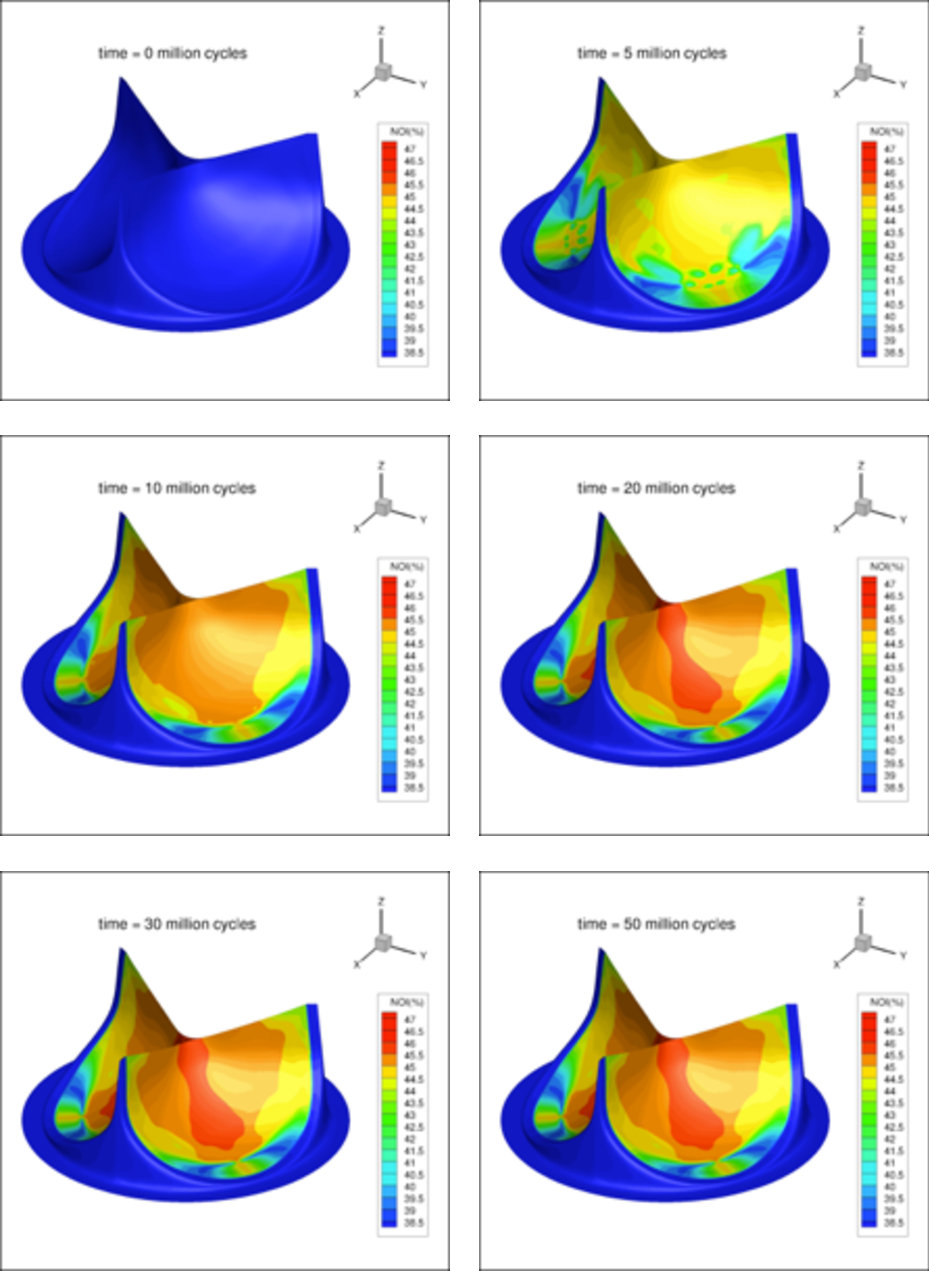
\includegraphics[width=5in]{Images/chapter6/permanentsetnoi.pdf}
\caption{The simulation of the evolution of the referential configuration with the normalized orientation index (NOI) overlayed, showing the changes in the degree of alignment of collagen fibers at different cycle levels. Higher NOI indicate higher aligned fiber orientation distributions.}
\label{c6:fig:psnoi}
\end{figure}
%-------------------	 end FIGURE 	-------------------%
%%%%%%%%%%%%%%%%%%%%%%%%%%%%%%%%%%%%%%%%%%%%%%%%%%%%%%%%%%%%
    
    Here we also note that the regions that undergo most permanent set are: the belly region, center of the free edge, and the regions near the commissures, where the leaflets initial makes contact (Fig. \ref{c6:fig:psdeformation}). These regions are also the most common regions of failure in BHVs. Due to the change in reference configuration, the collagen fibers in these regions recruit more quickly and may even held in a constant extended state. This can have dramatic consequences on the likelihood of failure of these collagen fibers due to their low extensibility, and could be a major mechanism for the fiber level damage in BHVs. 
    
    
    We have also shown that we can predict the change in the collagen fiber architecture (Fig. \ref{c6:fig:psnoi}). Here we plotted the normalized orientation index (NOI)
    \begin{equation}
        NOI = \frac{\sigma_iso - \sigma(s)}{\sigma_iso},
    \end{equation}
    which is based on how spread apart (standard deviation $\sigma$) is collagen fiber orientation is. Here, $NOI = 1$ indicate fully aligned distributions (delta distributions), which $NOI = 0$ indication that the fiber distribution is an uniform distribution. We can see that the belly region and the free edge undergoes the greatest degree of realignment. This is most likely due to the fact that these two regions receives the least amount of support from the neighboring leaflets. The most important aspect of being able to predict the structural changes is that we can use it to compute the degree of recruitment of collagen fibers in a similar method to chapter \ref{c2:sec:233}. This allows us to compute the distribution of collagen fiber by their stretches after being straightened. This mechanism can be used to potentially develop a strain-level dependent model for the likelihood of collagen fiber damage in a future extension. 

    


%---    Discussion
\section{Summary and Future Directions}
	We have developed the a complete time-dependent framework for the simulation of BHVs under long term cyclic loading. This simulation utilizes the predictive mechanism based constitutive model for the permanent set effect in exogenously crosslinked soft tissues that we previously developed. We have shown that we can use this simulation to predict the evolving geometry, microstructural and material property changes. These results can then be used to predict regions of increase likelihood of structural damage, and can be used to optimal the initial design of BHVs based on these factors. Most important of these effects is that the collagen fiber architecture can play a role in limiting the permanent set effect, where the straightening of collagen fibers prevents further changes in geometry. Thus, accounting for the permanent set effect is especially important in the design of BHVs to better improve their performance and durability. 
	
	
	The two main future extensions of this constitutive model and simulation is for: 1) structural damage and 2) growth and remodeling. Structural damage is difficult to quantify as it only gradually accumulates over long periods of time. Due to the exponential nature and large structural reserves of soft tissues, small decreases in the number or modulus of collagen fiber is very difficult to detect. This is also complicated by the fact that strain is difficult to quantify in the first place. In accelerated wear testing or other similar environments, this process is further complicate by the heterogeneity of the resulting response. However, by simulation and removing of the permanent set effect on the change in geometry, we can more accurately determine the remaining changes due to structural damage, This opens the doors to the development of mechanism-based structural damage models which is lack in literature. Growth and remodeling is a similar important future area, as this have important implications in prediction of the outcomes of diseases, injuries, and surgical interventions. The permanent set model and simulation framework developed herein is a simplification of the growth and remodeling framework by removing the growth component. This can have important potential implications is devices such as tissue engineered valves which have the possibility of growing and adaption to the surrounding environment if seeded with interstitial cells. 




%---    Bioliography
\bibliographystyle{plainnat}
\bibliography{phd}